\documentclass{standalone}
\usepackage{pgfplots}
\begin{document}
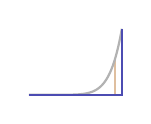
\begin{tikzpicture}
\pgfplotsset{width=3cm}
\begin{axis}[axis lines=none,scaled ticks=false,mark=none]
%\addplot[gray!100!white,domain=0:1,samples=201]{x^2};
%\addplot[gray!80!white,domain=0:1,samples=201]{x^4};
%\addplot[gray!60!white,domain=0:1,samples=201]{x^8};
\draw[brown!50!white, thick] (axis cs: {.93},0) -- (axis cs: {.93},{(.93)^8});
\addplot[gray!60!white,thick,domain=0:1,samples=201]{x^8};
%\addplot[gray!20!white,domain=0:1,samples=201]{x^(32)};
\draw[blue!40!gray,thick] (axis cs: 0,0) -- (axis cs: 1,0) -- (axis cs: 1,1);
\end{axis}
\end{tikzpicture}
\end{document}
